%%%%
\section{Fluorescência de Raios X}

Para determinação e quantificação das concentrações elemenares (número atômico $Z>10$)
foi utilizada a técnica não-destrutiva de \textit{Fluorescência de Raios X}.

\textit{Fluorescência de Raios X} é um método analítico quali-quantitativo, 
multielementar, que mede os raios-X característicos emitidos dos átomos da amostra, 
depois de também serem irradiados por Raios X. Não exige pré-tratamento químico
das amostras.

Existem 3 Tipos de fluorescências de raios X: dispersão em energia,
dispersão por comprimento de onda e reflexão total.
O usado nessa pesquisa foi o 
\textit{Fluorescência de Raios X por dispersão em energia}.

A figura \ref{fig:shimadzu_atomo} ilustra classicamente o que ocorre com
o átomo ao ser excitado.

\begin{figure}[H]
\begin{center} 
  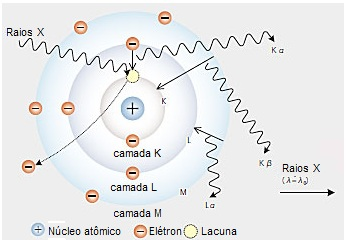
\includegraphics[width=0.5\textwidth]{../inputs/images/shimadzu_atomo.jpg}
  \caption{Shimadzu - Figura que acompanha o manual do XRF-ED \label{fig:shimadzu_atomo}}
   % http://www.shimadzu.com.br/analitica/produtos/elemental/raios_x/eds/images/edx-7000_8000-2.jpg
\end{center}
\end{figure}

O feixe de raios x incidente, neste caso produzido por tudo de raios X, 
expulsa os elétrons das camadas mais internas $K$ e $L$, produzindo vacâncias. 
Um átomo com vacância é instável e rapidamente elétrons das camadas 
mais externa preenchem as vacâncias estabilizando o átomo.

As transições dos elétrons das camadas mais externas para as camadas
$K$ e $L$ liberam Raios X característicos do átomo em questão. 

Transições da camada $L$ para $K$ são do tipo $K\alpha$, de $M$ para $K$ 
são $K\beta$ e de $M$ para $L$ são $L\alpha$ ou $L\beta$. 
A camada $L$ possue 3 e a camada $M$ 5 subníveis o que
resulta em inúmeras possibilidades de transições, sendo que algumas transições
proibidas. 

A \textit{notação de Siegbahn} permite identificarmos melhor os subníveis
de origen e destino, por exemplo, transição de $M_{IV}$ para $L_{III}$ é uma transição do 
tipo $L\beta_1$ \cite{jenkins1991}, outras possíveis pode ser vista na
figura \ref{fig:siegbahn}. 

\begin{figure}[H]
\begin{center} 
  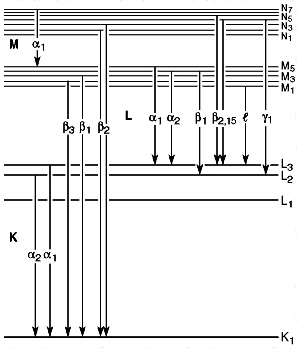
\includegraphics[width=0.5\textwidth]{../inputs/images/Siegbahn.jpg}
  \caption{Transições - artigo \cite{jenkins1991}  \label{fig:siegbahn}}
\end{center}
\end{figure}

Entretanto, há transições com energias são tão próximas 
que são indistinguiveis para os detectores (semicondutores) 
utilizados, sendo assim, neste trabalho vamos chamar apenas de 
transições tipo $K$ e $L$.

%%%%
\subsection{Fluorescência de Raios X por dispersão em energia}

A \textit{Fluorescência de Raios X por dispersão em energia} (\textbf{XRFED}).
usa detectores de semicondutores capaz de discriminar energia 
próximas, onde a distinção dos fótons é feita pela amplitude do pulso 
eletrônico produzido no detector, pois os pulsos eletrônicos são
proporcionais às energias dos raios X. 

O detector mais empregado é o de silício ativado com lítio $Si(Li)$.

A figura \ref{fig:esquemaxrfed} ilusta a geometria do \textbf{XRFED}. 

\begin{figure}[H]
\begin{center} 
  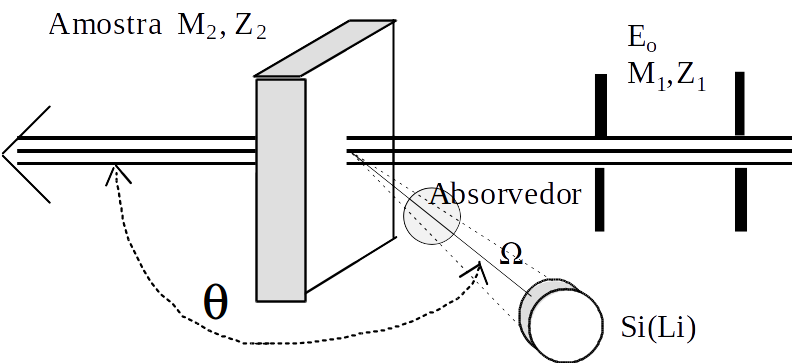
\includegraphics[width=0.5\textwidth]{../inputs/images/esquema-xrfed.png}
  \caption{Geometria de montagem fluorescência de Raios X por dispersão em energia \label{fig:esquemaxrfed}}
\end{center}
\end{figure}

E a figura \ref{fig:xrfed_iag} ...

\begin{figure}[H]
\begin{center}
  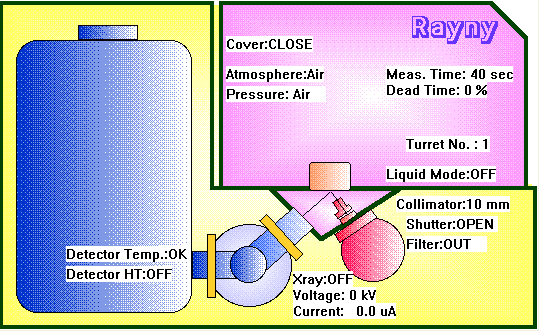
\includegraphics[scale=0.4]{../inputs/images/edx_iag_monitor.png}
  \caption{Fluorescência de Raios X por dispersão em energia do IAG USP - label{fig:xrfed_iag}}
\end{center}
\end{figure}

%%%%
\subsection{Calibração}

Energia de ligação pode ser aproximada pela teoria atômica de Bohr:
\begin{math}
E = \frac{me^4(Z-b)^2}{8w^2h^2n^2}
\end{math}

\begin{itemize}
  \item E = energia de ligação eletrônica (joules);
  \item m = massa de repouso do elétron = 9,11.10 -31 kilogramas;
  \item e = carga elétrica do elétron = 1,6.10 -19 coulombs;
  \item Z = número atômico do elemento emissor dos raios X;
  \item b = constante de Moseley, com valores iguais a 1 e 7,4, 
        para as camadas K e L, respectivamente;
  \item w = o = permitividade elétrica no vácuo = 8,8534.10 -12 
        coulombs.newton -l .metro -2;
  \item h = constante de Planck = 6,625.10 -34 joules.s;
  \item n = n o quântico principal do nível eletrônico 
        (n = 1 para camada K, n = 2 para camada L, etc.).
\end{itemize}

%86 # Y and X were measured
%187 # 
%188 # $[X]A=[Y]$
%189 # 
%190 # We will adjust a A for equation above and call it Ã, but before we have to calculate the covariance of the coeficients $V_Ã$:
%191 # 
%192 # $V_Ã = (X^T V_Y^{-1} X)^{-1}$
%193 # 
%194 # and
%195 # 
%1%96 # $Ã = V_Ã X^T V_Y^{-1} Y$
%197 # 
%198 # Now, we can calculate the new values of Y from $V_Ã$ to all atomic numbers in covered region $X_{adjusted}$:
%199 # 
%200 # $[X_{adjusted}]Ã=[Y_{adjusted}]$
%201 # 
%202 # The error desired is the square roots of diagonal of matrix covariance of Ycalculed $C_{Yadjusted}$.
%203 # 
%204 # $C_{Y_{adjusted}} = X_{adjusted} V_Ã X_{adjusted}^T$

\begin{equation}
\begin{split}
F = \{F_{x} \in  F_{c} &: (|S| > |C|) \\
 &\quad \cap (\text{minPixels}  < |S| < \text{maxPixels}) \\
 &\quad \cap (|S_{\text{conected}}| > |S| - \epsilon) \}
\end{split}
\end{equation}

%%%%
\subsection{Limite de Detecção}

Densidade mínima para haver detecção da espécie. % como determina para XRF?

Amostra espessas apresentam o efeito matriz, ou seja, interações dos 
raios X característicos com os elementos da amostras, causando 
absorção do raios X ou mesmo reforço de raios X.





